\chapter{Linear functions and slope}
%\addcontentsline{toc}{chapter}{1 Graphs}
%%%%%%%%%%%%%%% SECTION HEADER %%%%%%%%%%%%%%%%
\rhead{3}
\lhead{Linear functions and slope}
%%%%%%%%%%%%%%%%%%% START %%%$%%%%%%%%%%%%%%%%%
\section{Slope of a line}
The steepness or slope of a line in the $xy$-coordinate system is the ratio of the rise (the change in $y$-coordinates) to the run (the change in $x$-coordinates) between two points on the line. The slope is denoted as $m$. 
\begin{equation}
	m= \frac{\textit{Change in $y$}}{\textit{Change in $x$}} = \frac{Rise}{Run} = \frac{y_2-y_1}{x_2-x_1}
	 \label{slope}
\end{equation}
Notice the subscript 1 and 2 indicate first and second point, respectively.
\vspace{0.5cm}
\begin{center}
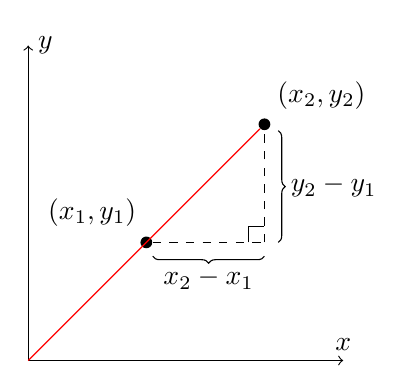
\begin{tikzpicture}
	\draw[->] (0,0) coordinate (O) -- (4,0) node[pos=1, above] {$x$};
	\draw[->] (O) -- (0,4) node[pos=1, right] {$y$};
	\node[inner sep=1.5pt,fill,circle,label={60:$(x_2,y_2)$}] 
    				at (3,3) (point2) {};
    \node[inner sep=1.5pt,fill,circle,label={93:$(x_1,y_1)$}] 
    				at (1.5,1.5) (point1) {};
	\draw[red] (0,0) -- (point2);
	\draw (2.8,1.5) -- ++(0,0.2) -- ++(0.2,0);
	\draw[dashed] (3,1.5) coordinate (pointx) -- (point2); 
    \draw[dashed] (point1) coordinate (pointx) -- (3,1.5); 
	\draw[decoration={brace,mirror,raise=5pt},decorate]
  	(3,1.5) -- node[right=6pt] {$y_2-y_1$} (point2);
	\draw[decoration={brace,mirror,raise=5pt},decorate]
  	(point1) -- node[below=6pt] {$x_2-x_1$} (3,1.5);
\end{tikzpicture}
\end{center}

\vspace{0.5cm}
In order to avoid any confusions, always label your points before using the \eqref{slope} formula. That way you wouldn't mix up their $x$- or $y$-coordinates.
% ======= EXAMPLE 1
\begin{exa}
 	Find the slope of the line passing through $(-3,3)$ and $(-5,7)$.
\end{exa}
First, Label our points.
\begin{align*}
		(-3,3)&	&&\text{Our first point, so $x_1=-3$ and $y_1=3$}\\
        (5,7)&  &&\text{Our second point, so $x_2=-5$ and $y_2=7$}
\end{align*}
Plug them into slope formula \eqref{slope} to find slope:
\begin{align*}
	m &=\frac{y_2-y_1}{x_2-x_1} \\
    m &=  \frac{7-3}{-5-(-3)} \\
    m &= \frac{4}{-2} \\
    m &= -2 \quad \text{Our solution}
\end{align*}
% =========SUBSECTION
\subsection{Slope of vertical and horizontal lines}
Imagine you are outside the classroom and walking on the ground. Since the ground doesn't have any steepness, you'd spend a minimum energy to walk; In fact, you prefer walking on the ground forever. On the other hand, you know as a mathematician, how hard would it to climb a precipitous cliff-almost impossible! \\
The ground is a horizontal line and since there is no steepness, the slope of horizontal line is 0. Likewise, the precipitous cliff is like a vertical line. Because it is impossible to climb the cliff-at least for mathematicians-the slope of a vertical line is undefined.
We can also prove this mathematically. Considering the vertical line, we know it passes through all points with the same $x$ coordinate. Using slope formula \eqref{slope}, we will get
\[
				m = \frac{y_2-y_1}{0}
\]
Since the denominator become zero and the slope is undefined. Let's consider horizontal line. The $y$ values of all points on a horizontal line are equal. Thus, using slope formula \eqref{slope}, we will get 
\[
				m = \frac{0}{x_2-x_1} =0
\]
zero divided by anything yields to zero. So, $m$ is zero.\\
We can also use "\textit{rise over run}" formula. In a vertical line, run is zero, so 
\[
						m=\frac{Rise}{0}
\]
which is undefined. However, in a horizontal line, there is no rise, 
so 
\[
						m=\frac{0}{Run}
\]
which gives us a zero slope.\newpage
Following graph summarize what we learned about the slope of the horizontal and vertical lines.
\begin{figure}[ht]
\centering
\begin{tikzpicture}
	\draw[->] (-3,0) -- (3,0) node[pos=1, above] {$x$};
	\draw[->] (0,-3) -- (0,3) node[pos=1, right] {$y$};
    \draw[<->, line width=0.3mm, red] (-2,-2.3) -- (-2,2.3);
    \node[label={\rotatebox{90}{slope is undefined}}] at (-2.5,-2) {};
    \draw[<->,line width=0.3mm, blue] (-1,1) -- (3,1);
    \node[label={slope is 0}] at (1.5,1) {};
\end{tikzpicture}
	\caption{Slope of a horizontal and vertical lines}
\end{figure}
% ======== SUBECTION
\subsection{Positive and negative slopes}
Lines sloping upward to the right have \textit{positive} slopes; In fact, if one end of line passes through quadrant I and the other end passes through quadrant III then slope is always positive.\\
On the other hand, lines sloping downward to the left have \textit{negative} slopes. In other words, a line with negative slope has one end at quadrant II and the other end at quadrant IV.
\begin{figure}[ht]
\centering
\begin{tikzpicture}
	\draw[->] (-2,0) -- (2,0) node[pos=1, above] {$x$};
	\draw[->] (0,-2) -- (0,2) node[pos=1, right] {$y$};
    \draw[<->, line width=0.3mm, red] (-1,1.5) -- (1.5,-1);
    \node[label={Negative slope}] at (0,-3) {};
\end{tikzpicture}
\quad
\begin{tikzpicture}
	\draw[->] (-2,0) -- (2,0) node[pos=1, above] {$x$};
	\draw[->] (0,-2) -- (0,2) node[pos=1, right] {$y$};
    \draw[<->,line width=0.3mm, blue] (-1.5,-1) -- (1,1.5);
    \node[label={Positive slopes}] at (0,-3) {};
\end{tikzpicture}
\caption{Negative and positive slopes}
\end{figure}
\section{Point-slope formula}
To find the equation of a line, we need to find a relationship between any $x$ and $y$ values on the line. Let's assume, we know the slope of a line, $m$, and we have one point on the line, $(x_1,y_1)$. Slope between any points on the line such as $(x,y)$ and our point $(x_1,y_1)$ should be
constant and equal to $m$. So using definition of slope, \eqref{slope}.
\begin{align*}
		\frac{y-y_1}{x-x_1} &=m &&\text{Multiply both sides by $(x-x_1)$}
        \\
        \cancel{(x-x_1)}\frac{y-y_1}{ \cancel{x-x_1}} &=m(x-x_1) 
        								&&\text{Simplify} \\
         y-y_1 &= m (x-x_1)			&&\text{Equation of the line} 
\end{align*}
This formula is called point-slope formula which is a general formula. We
will use this formula all the time to find the equation of any lines.
\begin{tcolorbox}[
                    title=Point-Slope formula,
                    fonttitle=\bfseries,
                    colframe=blue!70!red,
                    colback=white
                    ]
    If a line has a slope of $m$ and is passing through $(x_1,y_1)$ then
    the equation of the line is 
    	\begin{equation}
    				y-y_1 = m(x-x_1) \label{point_slope}
    	\end{equation}
\end{tcolorbox}
\begin{nt}
Since we need to find the linear function, we often need to solve for $y$ and then replace it with $f(x)$. This form is also called, \textbf{slop-intercept form} which we will discuss about it later in this section.
\end{nt}
% ======= EXAMPLE 2
\begin{exa}
	Write the equation of line through the point $(3, -4)$ with a slope of $6$. Then solve for the equations for $y$.
\end{exa}

We are given $m=6$ and $x_1=3, y_1=-4$. so
\begin{align*}
		y-y_1  &=m(x-x_1) &&\\
        y+4 &=6(x-3) &&\text{Our solution}
\end{align*}
Then we solve it for $y$
\begin{align*}
        y+4 =6(x-3)& &&\text{Distribute}\\
        y+4 =6x-18&    &&\text{Subtract 4 from both sides}\\
        y =6x-18-4&    &&\text{Simplify}\\
        y =6x-22&    &&\text{Our linear function}
\end{align*}
% =========

\vspace{0.4cm}
\begin{nt}
 Sometimes we want to find the equation of a line passing through \textbf{two points}. In this case, we first need to find the slope of the line. Then we use one of the point, and plug it into the point-slope formula to find the equation of our line.
\end{nt}
% ====== Example 3
\begin{exa}
	Find the equation of the line through the points $(2, 5)$ and 
    $(6, -3)$. Then solve the equation for $y$.
\end{exa}
\vspace{0.2 cm}
Label points and find the slope.
\begin{align*}
		(-2,1)&		&&\textrm{First point, $x_1=2$ and $y_1=5$}\\
        (4,5) &	&&\textrm{Second point, $x_2=6$ and $y_2=-3$}\\
        m = \frac{y_2-y_1}{x_2-x_1}&	&&\textrm{Slope formula}\\
        m = \frac{(-3)-(5)}{(6)-(2)}&	&&\textrm{Simplify}\\  
        m = \frac{-8}{4}&	&&\textrm{Reduce}\\
        m = -2&	&&\textrm{Our slope}
\end{align*}
Then I choose the first point, and plug it into the point-slope formula
\begin{align*}
		y-y_1 &= m(x-x_1) &&\\
        y-5 &= -2(x-2)	&&\textrm{Our solution}
\end{align*}
Now, solve the equation for $y$
\begin{align*}
        y-5 = -2(x-2)&	&&\text{Distribute}\\
        y-5 = -2x+4&    &&\text{Add 5 to both sides}\\
        y = -2x+4+5&    &&\text{Simplify}\\
        y = -2x+9&  &&\text{Our linear function}
\end{align*}
% ==================
\section{Slope-intercept form}
Sometimes we are given the slope $m$ but our given point is not any
ordinary point; it is $y$-intercept. Let's say the $y$-intercept
is $(0,b)$. By plugging them into point-slope formula \eqref{point_slope},
we'll get $y- b = m(x-0) $. Adding $b$ to both sides yields
\begin{equation}
			y = mx+ b\qquad or\qquad f(x)=mx+b \label{slope_intercept}\\
\end{equation}
This form is called \textit{the slope-intercept form}. There is only $y$ variable  on the left-hand (with coefficient 1). On the other side, we have $x$ and a constant.
% ======== EXAMPLE 2
\begin{exa}
	Write an equation of the line with slope $m=\frac{5}{6}$ and $y$-intercept $(0,-3)$.
\end{exa}
\vspace{0.2 cm}
Substitute into the slope-intercept form \eqref{slope_intercept}
\begin{align*}
            y = mx+ b&      &   &\text{The slope-intercept form}\\
			y = \frac{5}{6}x -3&    &   &\text{Our solution}
\end{align*}
% ==========
\vspace{0.2cm}
\begin{nt}
Slope-intercept form is the simplest and most important form. If the equation of a line is written in this form, then 
\begin{itemize}
	\item the coefficient of $x$ is our slope;
	\item the constant is the $y$-intercept.
\end{itemize}
For example, if we have $y=-\frac{4}{5}x-5$ we realize quickly that the slope of this line is $-\frac{4}{5}$ and its $y$-intercept is $(0,-5)$---without using any other formulas or graphs.
\end{nt}
% ==========
\section{General form}
Every line has a equation that can be expressed in the form
\begin{equation}
    			Ax+By+C=0 \label{general_form}
\end{equation}
Where $A, B, C \in \mathbb{R}$ and $A,B \neq 0$. This form is called the \textbf{general form}.\\
To find the slope and $y$-intercept of an equation of a line, we convert the general form to the slope-intercept form; This can be achieved by solving the general form for $y$. Once we found the slope-intercept form, the coefficient of $x$ is our slope and the constant is the $y$-intercept.

% ========= EXAMPLE 4
\begin{exa}
Find the slope and $y$-intercept of the equation: \[-3x-4y+8=0\]
\end{exa}
We begin by solving for $y$, so
\begin{align*}
		-3x-4y+8=0& && \text{Add $3x$ to both sides}\\
		-4y +8 =-3x&    &&\text{Subtract 8 from both sides}\\
        -4y = 3x-8& &&\text{Divide both sides by $-4$}\\
        y = \frac{3}{4}x-\frac{8}{4}&	&&\textrm{Simplify}\\
        y = \frac{3}{4}x -2&	&&\textrm{Slope-intercept form}
\end{align*}
The slope is the coefficient of $x$, so slope is $\frac{3}{4}$ and the constant is our $y$-intercept which is $(0,-2)$.
% ===========
\section{Graphing a linear function}
To graph a linear function, we at least need two points on the line. The simplest points, yet useful, are $x$- and $y$-intercept. To find the $x$-intercept, we set $y=0$ and solve for $x$. Similarly, to get the $y$-intercept, we set $x=0$ and find the $y$-value.\\
Once we found our intercepts, we plot them on $xy$-plane, and then connect them to get our line.\\
In short, draw a T-table like the following table and find $x$- and $y$-intercepts.
\begin{figure}[ht]
	\centering
    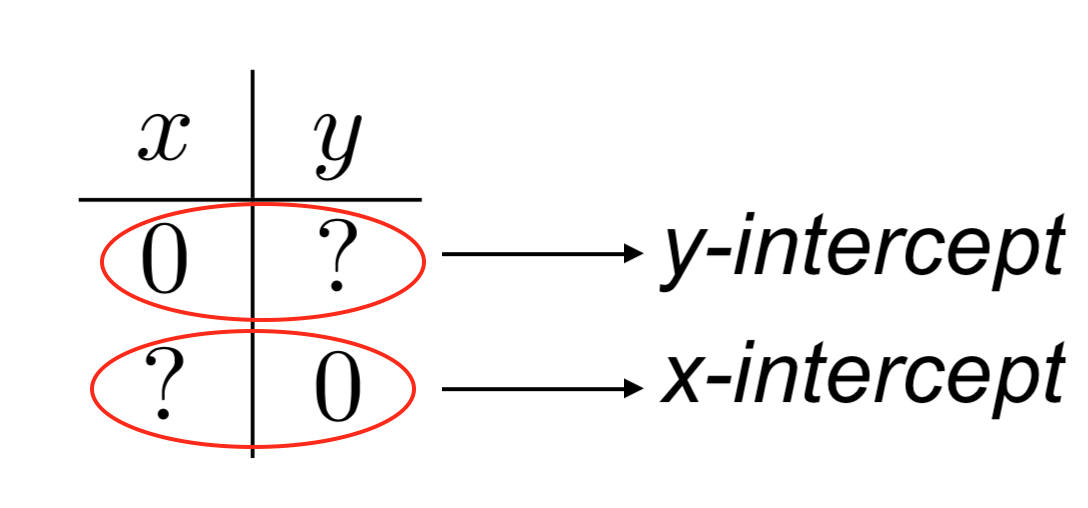
\includegraphics[width=5cm]{Pics/table_intercept.png}
\end{figure}
% ======== EXAMPLE 6
\begin{exa}
	Graph the equation $y=-4x+2$.
\end{exa}
To find the $y$-intercept, we set $x=0$ thus
\begin{align*}
		y =-4(0)+2& &   &\text{Plug $x=0$} \\
        y = 2& &&\text{$y$-intercept}
\end{align*}
For $x$-intercept, set $y=0$ and solve for $x$
\begin{align*}
		0 = -4x+2&  &&\text{Plug $y=0$} \\
        -2  =-4x& && \\
        \frac{1}{2}  = x& &&\text{$x$-intercept}
\end{align*}
Our table of values becomes like this
\begin{center}
\begin{tabular}{ c | c }
    $x$ & $y$ \\ \hline
    0	&  2 \\
    $\displaystyle \frac{1}{2}$   &  0  
\end{tabular}
\end{center}
Therefore our first point on the line is $(0,2)$ and the second one is $\left(\frac{1}{2}, 0\right) $. Plot these points and connect them to get the line.
\begin{center}
\begin{tikzpicture}
	\begin{axis}[my style,
    minor tick num=1,
	xmin=-3, xmax=3, ymin=-3, ymax=3]
	\addplot[domain=-3:3] {-4*x+2};
    \addplot[mark=*] coordinates {(0,2)};
    \addplot[mark=*] coordinates {(0.5,0)};
    \node[red, scale=0.9] at (-1.5,1) () {$y=-4x+2$};
	\end{axis}
\end{tikzpicture}
\end{center}
% ============
\subsection{Vertical and horizontal lines}
The graph of the equation $x=h$, where $h$ is any real number, is a vertical line through the point $(h,0)$.\\
To graph a vertical line, locate $x=h$ on $x$-axis and then draw a vertical line passing through it. The following graph, for example, shows the line $x=-2$.

\vspace{0.4cm}
\begin{figure}[ht]
\centering
\begin{tikzpicture}
	\begin{axis}[my style,
    minor tick num=1,
	xmin=-3, xmax=3, ymin=-3, ymax=3]
    \addplot +[<->, ultra thick, mark=none] coordinates {(-2, -3) (-2, 3)};
    \end{axis}
\end{tikzpicture}
    \caption{Graph of $x=-2$.}
\end{figure}
\vspace{0.4cm}
On contrary, the graph of the equation $y=k$, where $k$ is any real number, represents a horizontal line through the point $(0,k)$.\\
To graph a horizontal line, locate $y=k$ on the $y$-axis and then draw a horizontal line passing though it. For instance, the following graph shows the horizontal line $y=1$. 
\begin{figure}[ht]
\centering
\begin{tikzpicture}
	\begin{axis}[my style,
    minor tick num=1,
	xmin=-3, xmax=3, ymin=-3, ymax=3]
  	\addplot[<->, mark=none, ultra thick, red, domain=-2.7:2.7] {1};
  	\end{axis}
\end{tikzpicture}
\caption{Graph of $y=1$}
\end{figure}

\newpage
As you might remember, the slope of a vertical line is not defined and the slope of a horizontal line is always 0.
